\section{theorem12(the main theorem)}
\begin{theorem}
\end{theorem}

Generator Move\\

Suppose we have a Riemann sphere and a natural alternating diagram and a local system on the associated conjugate surface which could be represented as a sheaf $\mathfrak{F}$ singular supported along the natural alternating strand diagram.\\
Suppose the sheaf $\mathfrak{F}$ restricted to the generator region $D\subset C$ is as follows :

\begin{figure}[H] % Optional: [h] means here, [t] for top, [b] for bottom, [p] for page of floats
    \centering
    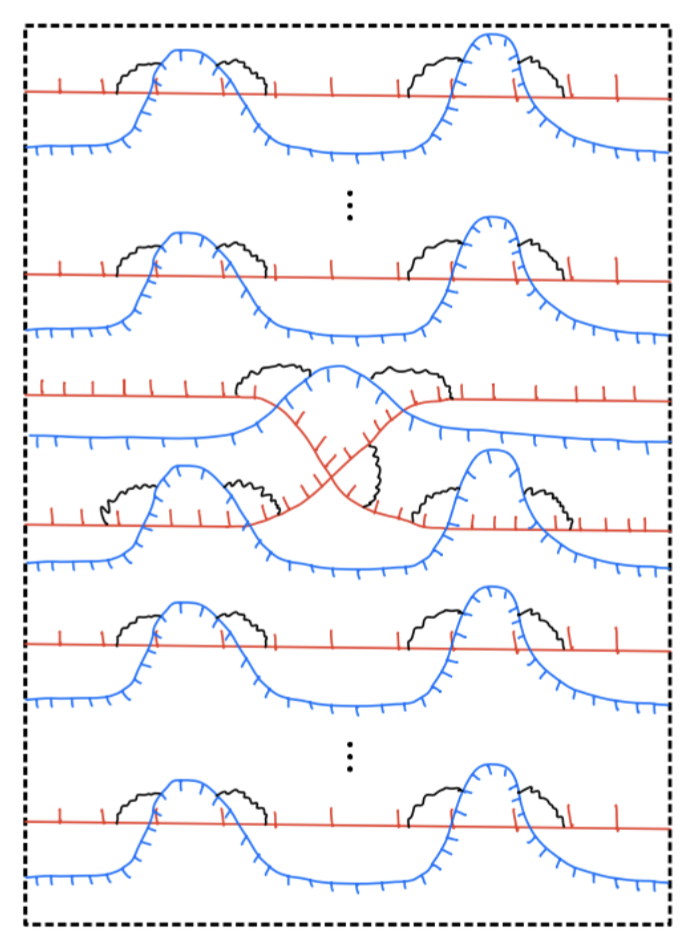
\includegraphics[width=\linewidth]{diagrams/theorem12/1.png} % Adjust the width as needed
    \caption{Your caption here}
    \label{fig:your-label}
\end{figure}
Let the $l^{th}$ crossing from the left of the $j^{th}$ blue strand be $c_{j,l}$.\\
- If $j\neq i$, there are $c_{j,1},c_{j,2},c_{j,3},c_{j,4}$\\
- If $j= i$, there are $c_{j,1},c_{j,2}$\\

Stalks:\\
- $N_{j,1}$ : $\mathbb{C}$\\
- $W_{j,1}$ : $0$\\
- $E_{j,1}$ : $\mathbb{C}\xrightarrow{\times a_j} \mathbb{C}$\\
- $S_{j,1}$ : $\mathbb{C}[-1]$\\
- $N_{j,2}$ : $\mathbb{C}$\\
- $W_{j,2}$ : $\mathbb{C}\xrightarrow{\times b_j} \mathbb{C}$\\
- $E_{j,2}$ : $0$\\
- $S_{j,2}$ : $\mathbb{C}[-1]$\\
- $N_{j,3}$ : $\mathbb{C}$\\
- $W_{j,3}$ : $0$\\
- $E_{j,3}$ : $\mathbb{C}\xrightarrow{\times c_j} \mathbb{C}$\\
- $S_{j,3}$ : $\mathbb{C}[-1]$\\
- $N_{j,4}$ : $\mathbb{C}$\\
- $W_{j,4}$ : $\mathbb{C}\xrightarrow{\times d_j} \mathbb{C}$\\
- $E_{j,4}$ : $0$\\
- $S_{j,4}$ : $\mathbb{C}[-1]$\\

Let the crossing of $i^{th}$ and $i+1^{th}$ red strands be mc, then \\

- $N$ : $\mathbb{C}$\\
- $E$ : $\mathbb{C}\xrightarrow{\times c}\mathbb{C}$\\
- $W$ : $0$\\
- $S$ : $\mathbb{C}[-1]$\\

Generization maps :\\
- $S_{j,1} \rightarrow E_{j,1}$ : 
\begin{tikzcd}
\mathbb{C} \arrow[r,"id"]     & \mathbb{C}  \\
0 \arrow[r,]\arrow[u,] & \mathbb{C} \arrow[u,"\times a_j"]
\end{tikzcd}
\\
- $E_{j,1}\rightarrow N_{j,1}$ : 
\begin{tikzcd}
\mathbb{C} \arrow[r,]     & 0  \\
\mathbb{C} \arrow[r,"id"]\arrow[u,"\times a_j"] & \mathbb{C} \arrow[u,]
\end{tikzcd}
\\
- $S_{j,2} \rightarrow W_{j,2}$ : 
\begin{tikzcd}
\mathbb{C} \arrow[r,"id"]     & \mathbb{C}  \\
0 \arrow[r,]\arrow[u,] & \mathbb{C} \arrow[u,"\times b_j"]
\end{tikzcd}
\\
- $W_{j,2}\rightarrow N_{j,2}$ : 
\begin{tikzcd}
\mathbb{C} \arrow[r,]     & 0  \\
\mathbb{C} \arrow[r,"id"]\arrow[u,"\times b_j"] & \mathbb{C} \arrow[u,]
\end{tikzcd}
\\
- $S_{j,3} \rightarrow E_{j,3}$ : 
\begin{tikzcd}
\mathbb{C} \arrow[r,"id"]     & \mathbb{C}  \\
0 \arrow[r,]\arrow[u,] & \mathbb{C} \arrow[u,"\times c_j"]
\end{tikzcd}
\\
- $E_{j,3}\rightarrow N_{j,3}$ : 
\begin{tikzcd}
\mathbb{C} \arrow[r,]     & 0  \\
\mathbb{C} \arrow[r,"id"]\arrow[u,"\times c_j"] & \mathbb{C} \arrow[u,]
\end{tikzcd}
\\
- $S_{j,4} \rightarrow W_{j,4}$ : 
\begin{tikzcd}
\mathbb{C} \arrow[r,"id"]     & \mathbb{C}  \\
0 \arrow[r,]\arrow[u,] & \mathbb{C} \arrow[u,"\times d_j"]
\end{tikzcd}
\\
- $W_{j,4}\rightarrow N_{j,4}$ : 
\begin{tikzcd}
\mathbb{C} \arrow[r,]     & 0  \\
\mathbb{C} \arrow[r,"id"]\arrow[u,"\times d_j"] & \mathbb{C} \arrow[u,]
\end{tikzcd}
\\
rest of the maps are zero maps.

Now we will define a move called "generator move" to $\mathfrak{F}$ so that the final sheaf is as follows :\\
\begin{figure}[H] % Optional: [h] means here, [t] for top, [b] for bottom, [p] for page of floats
    \centering
    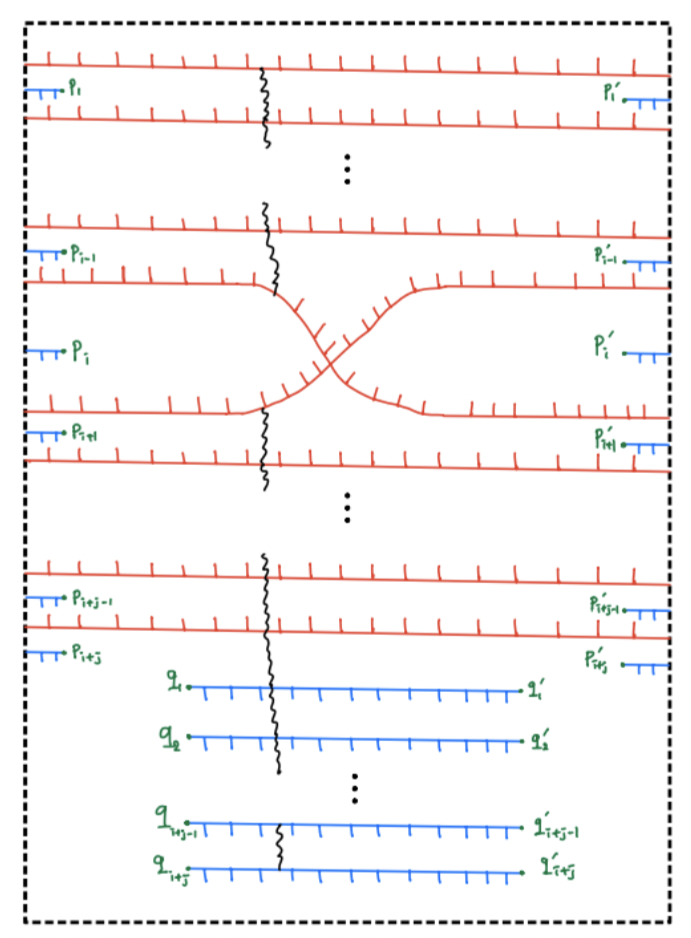
\includegraphics[width=\linewidth]{diagrams/theorem12/2.png} % Adjust the width as needed
    \caption{Your caption here}
    \label{fig:your-label}
\end{figure}



Here I intentionally omitted lines connecting:\\
- $p_l$ and $q_l$\\
- $p'_l$ and $q'_l$\\

do as not to make diagram too messy.\\

Let's denote the crossing of $p_{l_1},q_{l_1}$($p'_{l_1},q'_{l_1}$ resp.) with $l_2^th$ red strand as $c_{l_1,l_2}$($c'_{l_1,l_2}$ resp.).\\

Let's denote the north, east, west, south of $c_{l_1,l_2}$($c'_{l_1,l_2}$ resp.) as $N_{l_1,l_2}, E_{l_1,l_2}, W_{l_1,l_2},S_{l_1,l_2}$($N'_{l_1,l_2}, E'_{l_1,l_2}, W'_{l_1,l_2},S'_{l_1,l_2}$ resp.)\\

The final sheaf $\mathfrak{F}'$ can be described as follows:\\

Stalks:\\
- $N_{l_1,l_2}$ : $\mathbb{C}^{l_2 -l_1 +1}$\\
- $W_{l_1,l_2}$ : $\mathbb{C}^{l_2 -l_1}$\\
- $E_{l_1,l_2}$ : $\mathbb{C}^{l_2 -l_1}$\\
- $S_{l_1,l_2}$ : $\mathbb{C}^{l_2 -l_1 -1}$\\
- the stalk of the upper-most and bottom-most regions are $0$\\

Generization maps:\\
- $W_{1,l_2}\rightarrow E'_{1,l_2}$ : if $l_2\geq 2$ and $l_2 \neq i,i+1$,

$
\begin{pmatrix}
		\begin{matrix} 
			u_{1} & \cdots & 0 \\ 
			\vdots & \ddots & \vdots\\
			0 & \cdots & u_{i-1}
		\end{matrix} & \vline &
		\begin{matrix}
			0&0\\
			\vdots&\vdots\\
			0&0
		\end{matrix}& \vline &
		\begin{matrix} 
			0 & \cdots & 0 \\ 
			\vdots & \ddots & \vdots\\
			0 & \cdots & 0
		\end{matrix}\\
		\hline
		\begin{matrix}
			0&\cdots&0\\
			0&\cdots&0
		\end{matrix}z
		& \vline &
		\begin{matrix}
			\alpha & 0\\
			\beta & v_1
		\end{matrix} & \vline&
		\begin{matrix}
			0&\cdots&0\\
			0&\cdots&0
		\end{matrix}\\
		\hline
		\begin{matrix} 
			0 & \cdots & 0 \\ 
			\vdots & \ddots & \vdots\\
			0 & \cdots & 0
		\end{matrix} & \vline &
		\begin{matrix}
			0&0\\
			\vdots&\vdots\\
			0&0
		\end{matrix}& \vline &
		\begin{matrix} 
			v_2 & \cdots & 0 \\ 
			\vdots & \ddots & \vdots\\
			0 & \cdots & v_{j-1}
		\end{matrix}
		
\end{pmatrix}_{1,l_2 -1}
$\\
- $W_{1,i}\rightarrow E'_{1,i+1}$ : 

$
\begin{pmatrix}
		\begin{matrix} 
			u_{1} & \cdots & 0 \\ 
			\vdots & \ddots & \vdots\\
			0 & \cdots & u_{i-1}
		\end{matrix} & \vline &
		\begin{matrix}
			0&0\\
			\vdots&\vdots\\
			0&0
		\end{matrix}& \vline &
		\begin{matrix} 
			0 & \cdots & 0 \\ 
			\vdots & \ddots & \vdots\\
			0 & \cdots & 0
		\end{matrix}\\
		\hline
		\begin{matrix}
			0&\cdots&0\\
			0&\cdots&0
		\end{matrix}z
		& \vline &
		\begin{matrix}
			\alpha & 0\\
			\beta & v_1
		\end{matrix} & \vline&
		\begin{matrix}
			0&\cdots&0\\
			0&\cdots&0
		\end{matrix}\\
		\hline
		\begin{matrix} 
			0 & \cdots & 0 \\ 
			\vdots & \ddots & \vdots\\
			0 & \cdots & 0
		\end{matrix} & \vline &
		\begin{matrix}
			0&0\\
			\vdots&\vdots\\
			0&0
		\end{matrix}& \vline &
		\begin{matrix} 
			v_2 & \cdots & 0 \\ 
			\vdots & \ddots & \vdots\\
			0 & \cdots & v_{j-1}
		\end{matrix}
		
\end{pmatrix}_{1,i -1}
$\\
- $N_{l_1,i+j}\rightarrow N'_{l_1,i+j}$ : 

$
\begin{pmatrix}
		\begin{matrix} 
			u_{1} & \cdots & 0 \\ 
			\vdots & \ddots & \vdots\\
			0 & \cdots & u_{i-1}
		\end{matrix} & \vline &
		\begin{matrix}
			0&0\\
			\vdots&\vdots\\
			0&0
		\end{matrix}& \vline &
		\begin{matrix} 
			0 & \cdots & 0 \\ 
			\vdots & \ddots & \vdots\\
			0 & \cdots & 0
		\end{matrix}\\
		\hline
		\begin{matrix}
			0&\cdots&0\\
			0&\cdots&0
		\end{matrix}z
		& \vline &
		\begin{matrix}
			\alpha & 0\\
			\beta & v_1
		\end{matrix} & \vline&
		\begin{matrix}
			0&\cdots&0\\
			0&\cdots&0
		\end{matrix}\\
		\hline
		\begin{matrix} 
			0 & \cdots & 0 \\ 
			\vdots & \ddots & \vdots\\
			0 & \cdots & 0
		\end{matrix} & \vline &
		\begin{matrix}
			0&0\\
			\vdots&\vdots\\
			0&0
		\end{matrix}& \vline &
		\begin{matrix} 
			v_2 & \cdots & 0 \\ 
			\vdots & \ddots & \vdots\\
			0 & \cdots & v_{j-1}
		\end{matrix}
		
\end{pmatrix}_{l_1,i+j}
$\\
- $E'_{1,i+1}\rightarrow E_{1,i+1}$ : 
$
\begin{pmatrix}
		\begin{matrix} 
			u_{1}^{-1} & \cdots & 0 \\ 
			\vdots & \ddots & \vdots\\
			0 & \cdots & u_{i-1}^{-1}
		\end{matrix}\\
		\hline
		\begin{matrix}
			0&\cdots&0
		\end{matrix}
\end{pmatrix}
$\\
\\
- $E_{1,i+1}\rightarrow E'_{1,i+2}$ : 
$
\begin{pmatrix}
		\begin{matrix} 
			u_{1} & \cdots & 0 \\ 
			\vdots & \ddots & \vdots\\
			0 & \cdots & u_{i-1}
		\end{matrix} & \vline &
		\begin{matrix}
			0\\
			\vdots\\
			0
		\end{matrix}\\
		\hline
		\begin{matrix}
			0&\cdots&0\\
			0&\cdots&0
		\end{matrix}
		& \vline &
		\begin{matrix}
			\alpha\\
			\beta
		\end{matrix}
\end{pmatrix}
$\\

- All the other maps crossing the blue strands are $\iota_l$.\\
- All the other maps crossing the red strands are $\iota_f$.\\
- Rest of the maps are zero maps.\\

Now let's define the "Generator move" step by step.\\

(step1) Apply $Move_2$ to the disk surrounded by purple dotted lines:

\begin{figure}[H] % Optional: [h] means here, [t] for top, [b] for bottom, [p] for page of floats
    \centering
    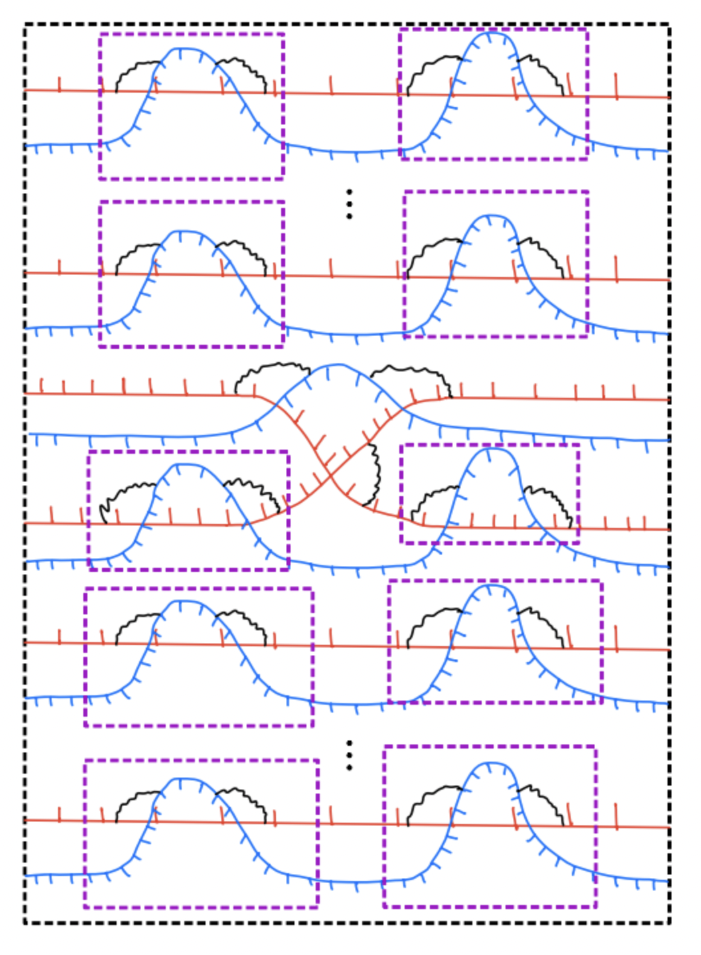
\includegraphics[width=\linewidth]{diagrams/theorem12/3.png} % Adjust the width as needed
    \caption{Your caption here}
    \label{fig:your-label}
\end{figure}

We get the following diagram:
\begin{figure}[H] % Optional: [h] means here, [t] for top, [b] for bottom, [p] for page of floats
    \centering
    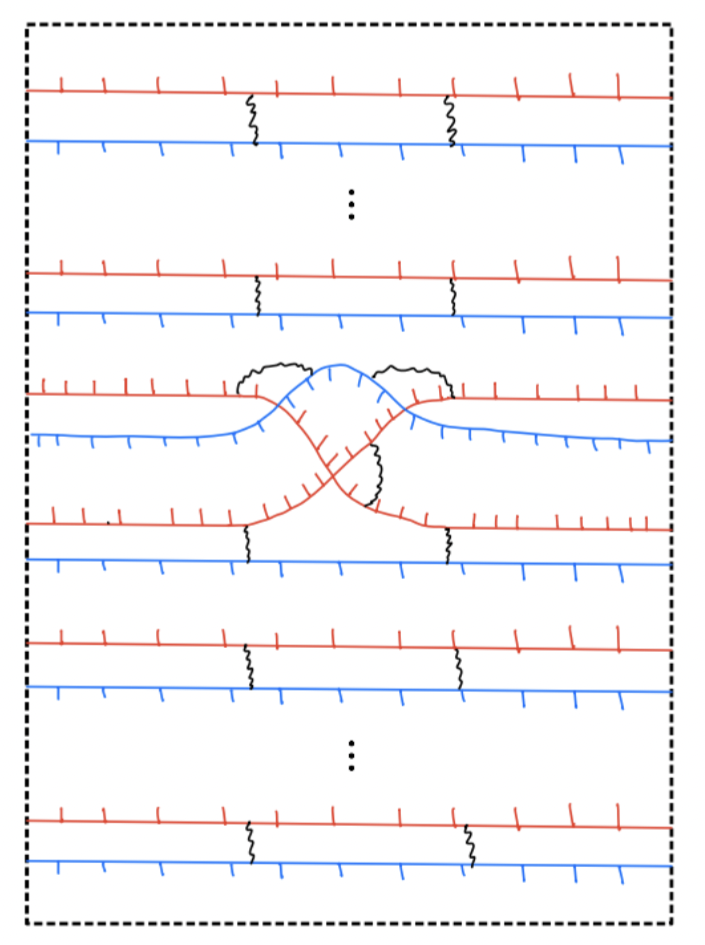
\includegraphics[width=\linewidth]{diagrams/theorem12/4.png} % Adjust the width as needed
    \caption{Your caption here}
    \label{fig:your-label}
\end{figure}

(Step2) Now change the basis of the stalks of the regions containing purple start so that the map corresponding to the squiggly lines to the right of the stars are identity maps:
\begin{figure}[H] % Optional: [h] means here, [t] for top, [b] for bottom, [p] for page of floats
    \centering
    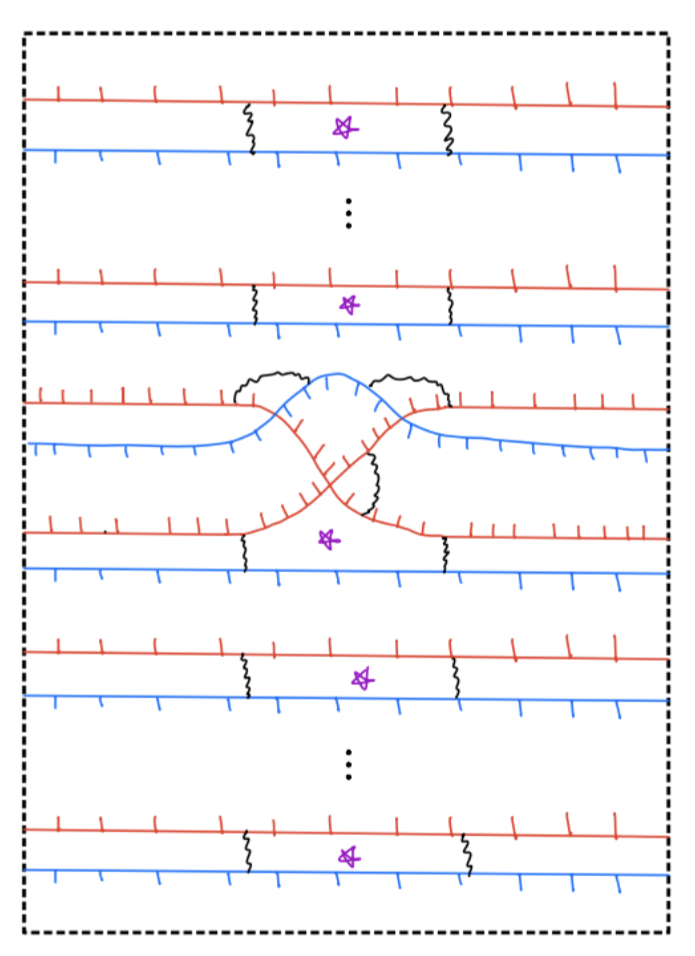
\includegraphics[width=\linewidth]{diagrams/theorem12/5.png} % Adjust the width as needed
    \caption{Your caption here}
    \label{fig:your-label}
\end{figure}

We get the following diagram:

\begin{figure}[H] % Optional: [h] means here, [t] for top, [b] for bottom, [p] for page of floats
    \centering
    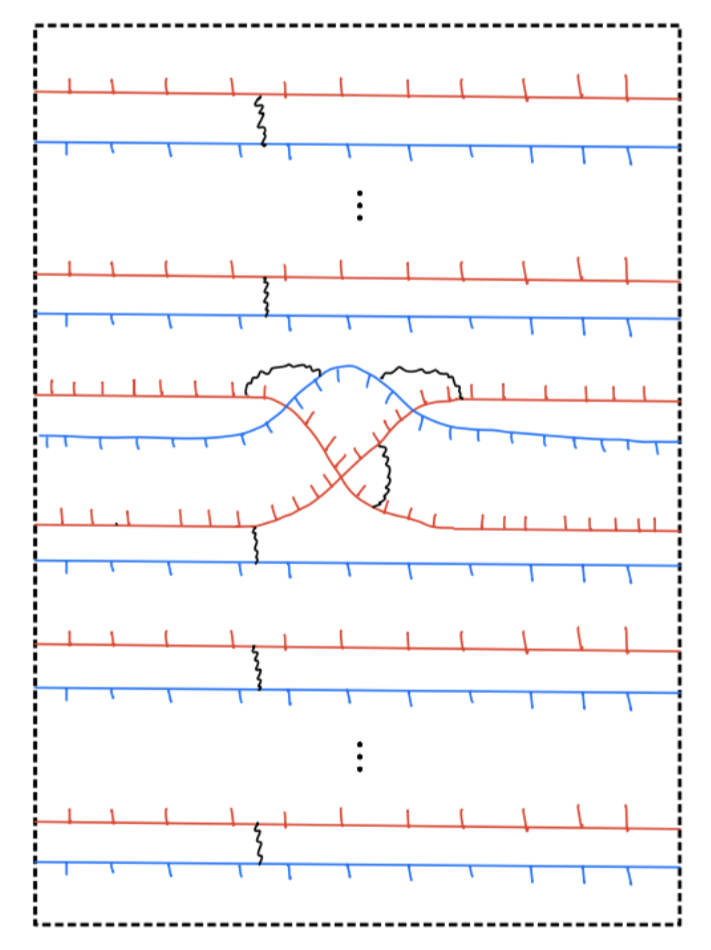
\includegraphics[width=\linewidth]{diagrams/theorem12/6.png} % Adjust the width as needed
    \caption{Your caption here}
    \label{fig:your-label}
\end{figure}

(Step3) Now we apply $Move_{7-(a)}$ to the disks surrounded by purple dotted lines:

\begin{figure}[H] % Optional: [h] means here, [t] for top, [b] for bottom, [p] for page of floats
    \centering
    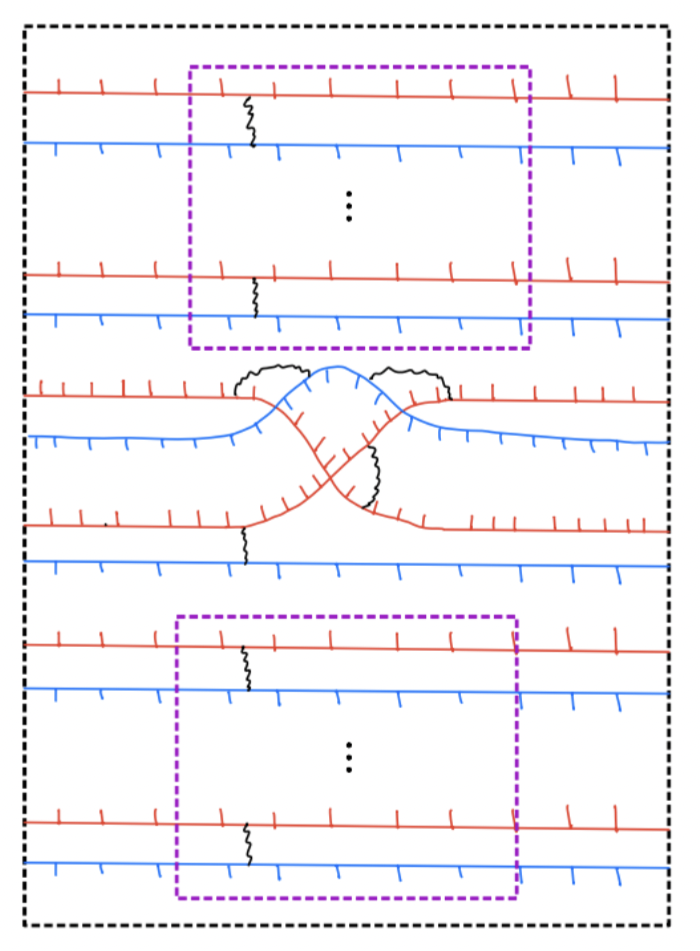
\includegraphics[width=\linewidth]{diagrams/theorem12/7.png} % Adjust the width as needed
    \caption{Your caption here}
    \label{fig:your-label}
\end{figure}

We get the following diagram:

\begin{figure}[H] % Optional: [h] means here, [t] for top, [b] for bottom, [p] for page of floats
    \centering
    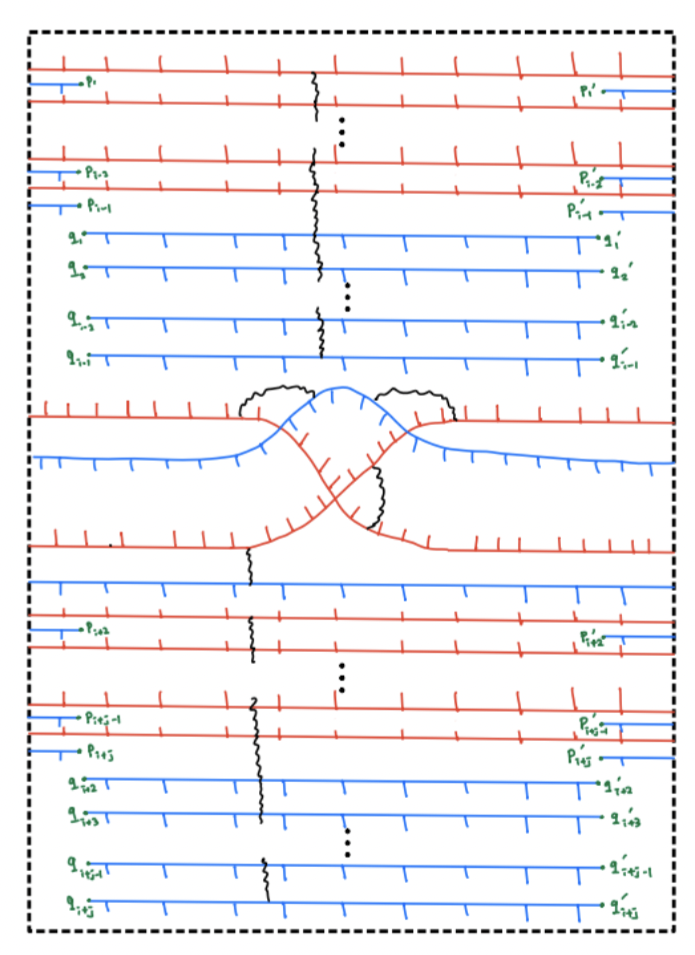
\includegraphics[width=\linewidth]{diagrams/theorem12/8.png} % Adjust the width as needed
    \caption{Your caption here}
    \label{fig:your-label}
\end{figure}

(Step4) Now we apply $Move_{7-(b)}$ to the disks surrounded by purple dotted lines:

\begin{figure}[H] % Optional: [h] means here, [t] for top, [b] for bottom, [p] for page of floats
    \centering
    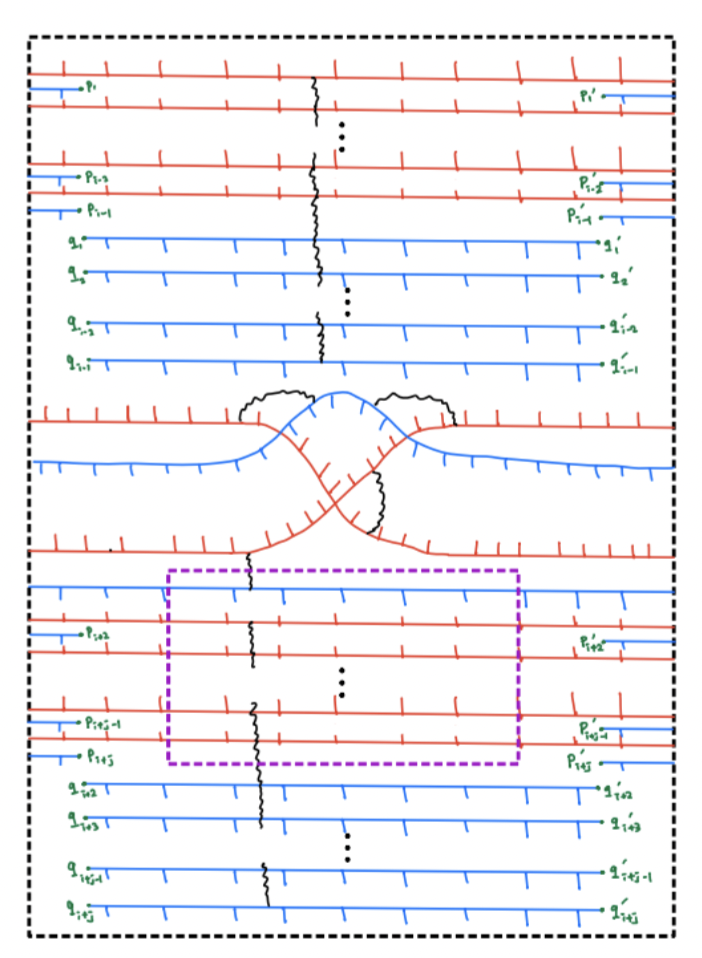
\includegraphics[width=\linewidth]{diagrams/theorem12/9.png} % Adjust the width as needed
    \caption{Your caption here}
    \label{fig:your-label}
\end{figure}

We get the following diagram:

\begin{figure}[H] % Optional: [h] means here, [t] for top, [b] for bottom, [p] for page of floats
    \centering
    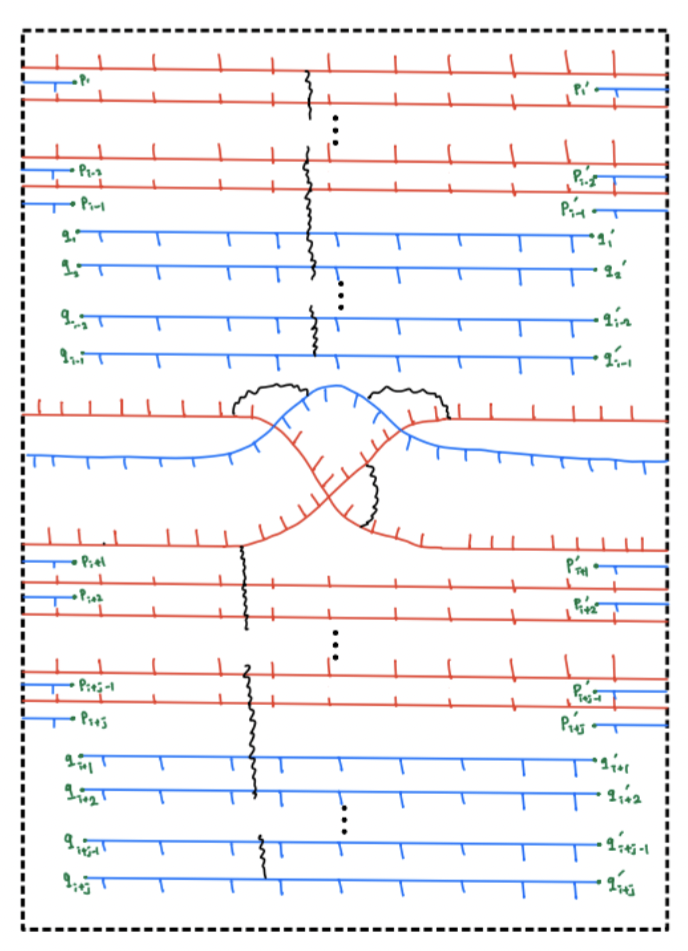
\includegraphics[width=\linewidth]{diagrams/theorem12/10.png} % Adjust the width as needed
    \caption{Your caption here}
    \label{fig:your-label}
\end{figure}

(Step5) Now we apply $Move_9$ to the disks surrounded by purple dotted lines:

\begin{figure}[H] % Optional: [h] means here, [t] for top, [b] for bottom, [p] for page of floats
    \centering
    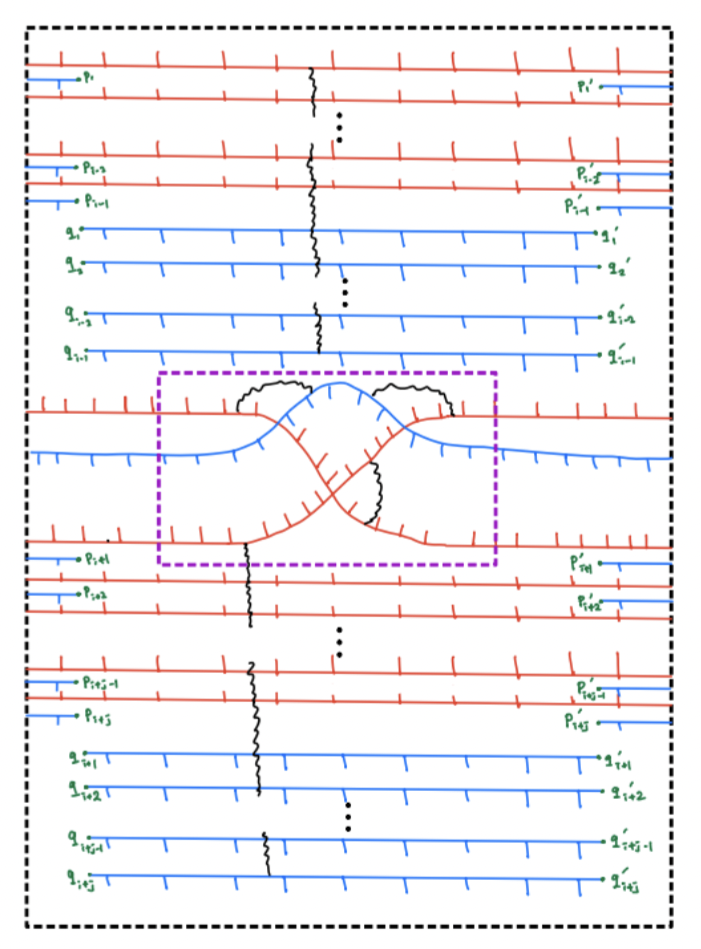
\includegraphics[width=\linewidth]{diagrams/theorem12/11.png} % Adjust the width as needed
    \caption{Your caption here}
    \label{fig:your-label}
\end{figure}

We get the following diagram:

\begin{figure}[H] % Optional: [h] means here, [t] for top, [b] for bottom, [p] for page of floats
    \centering
    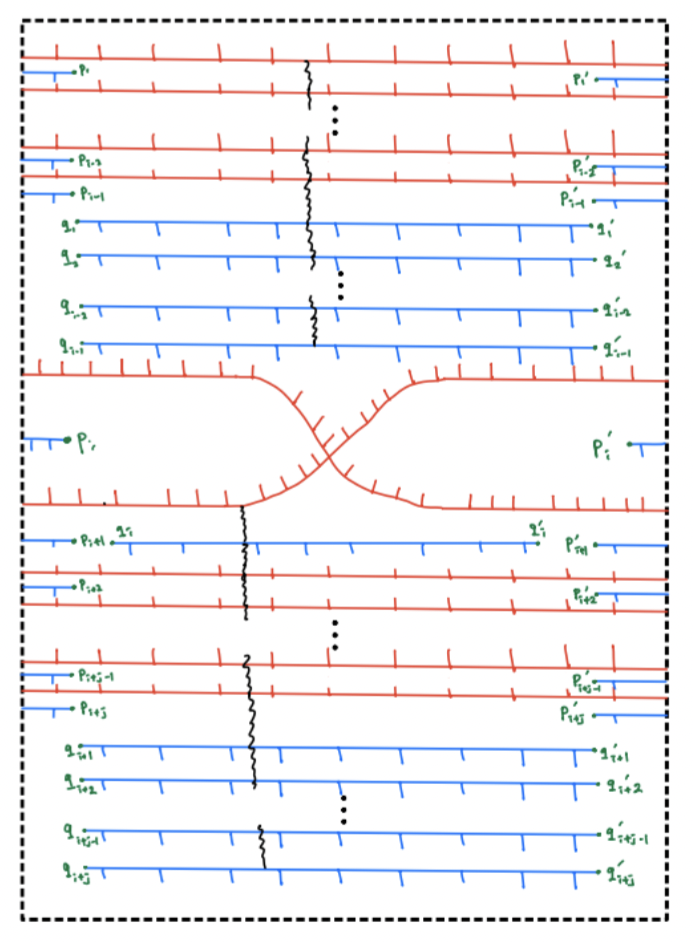
\includegraphics[width=\linewidth]{diagrams/theorem12/12.png} % Adjust the width as needed
    \caption{Your caption here}
    \label{fig:your-label}
\end{figure}

(Step6) Now we apply $Move_{11}$ to the disks surrounded by purple dotted lines:

\begin{figure}[H] % Optional: [h] means here, [t] for top, [b] for bottom, [p] for page of floats
    \centering
    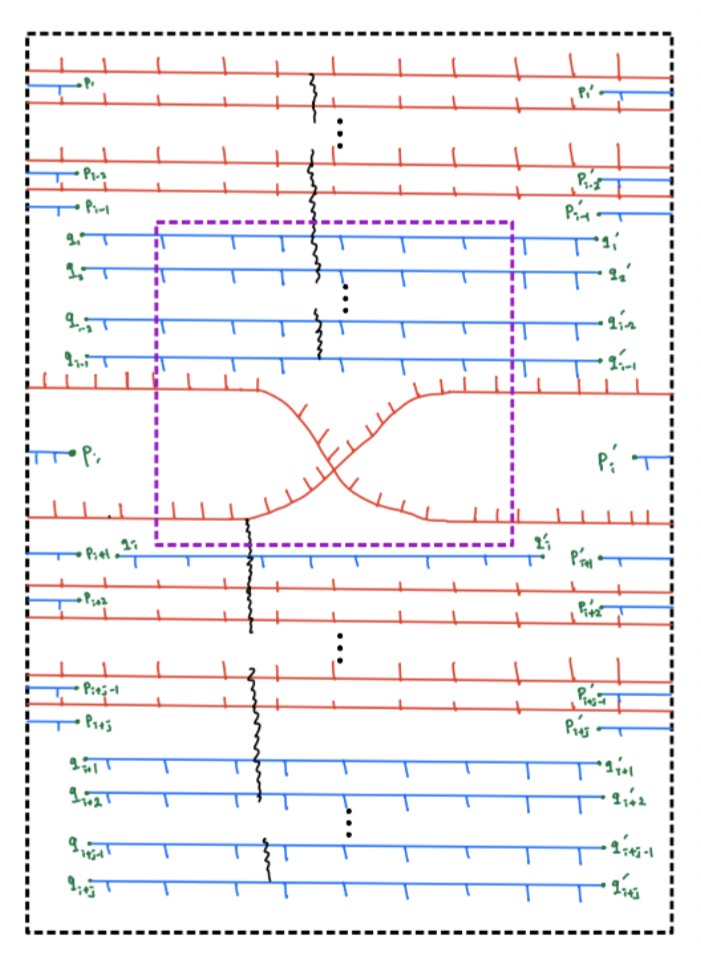
\includegraphics[width=\linewidth]{diagrams/theorem12/13.png} % Adjust the width as needed
    \caption{Your caption here}
    \label{fig:your-label}
\end{figure}

We get the following diagram:

\begin{figure}[H] % Optional: [h] means here, [t] for top, [b] for bottom, [p] for page of floats
    \centering
    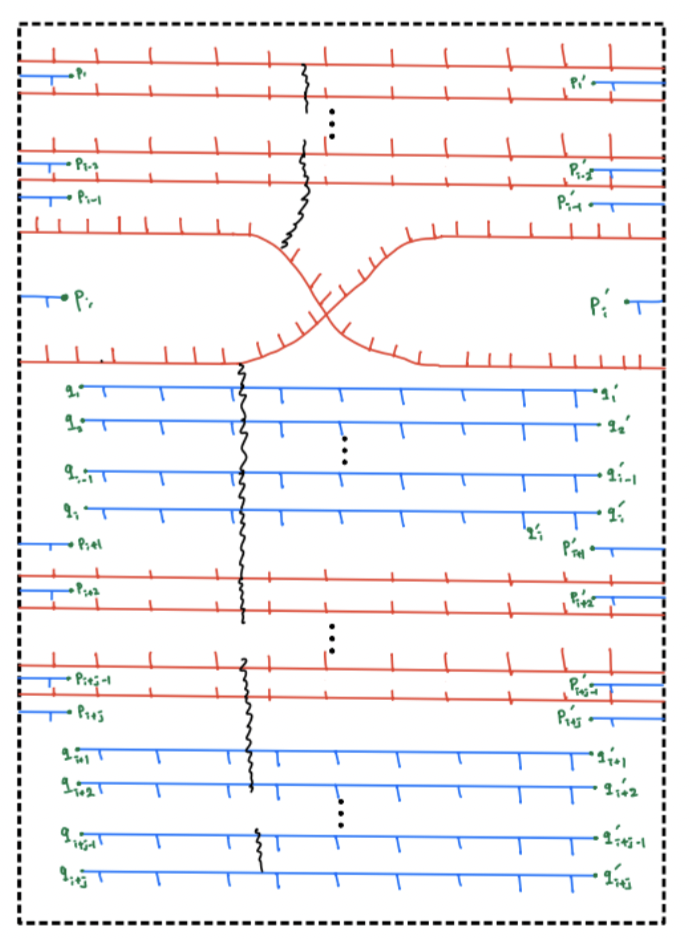
\includegraphics[width=\linewidth]{diagrams/theorem12/14.png} % Adjust the width as needed
    \caption{Your caption here}
    \label{fig:your-label}
\end{figure}

(Step7) Now we apply $Move_{7-(b)}$ to the disks surrounded by purple dotted lines:

\begin{figure}[H] % Optional: [h] means here, [t] for top, [b] for bottom, [p] for page of floats
    \centering
    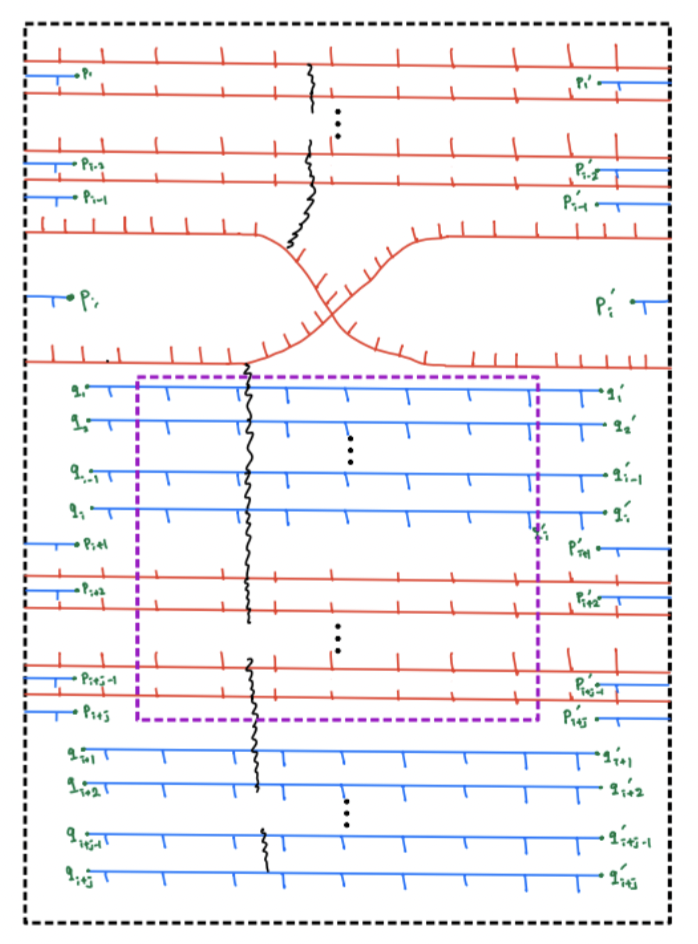
\includegraphics[width=\linewidth]{diagrams/theorem12/15.png} % Adjust the width as needed
    \caption{Your caption here}
    \label{fig:your-label}
\end{figure}

We get the final diagram:

\begin{figure}[H] % Optional: [h] means here, [t] for top, [b] for bottom, [p] for page of floats
    \centering
    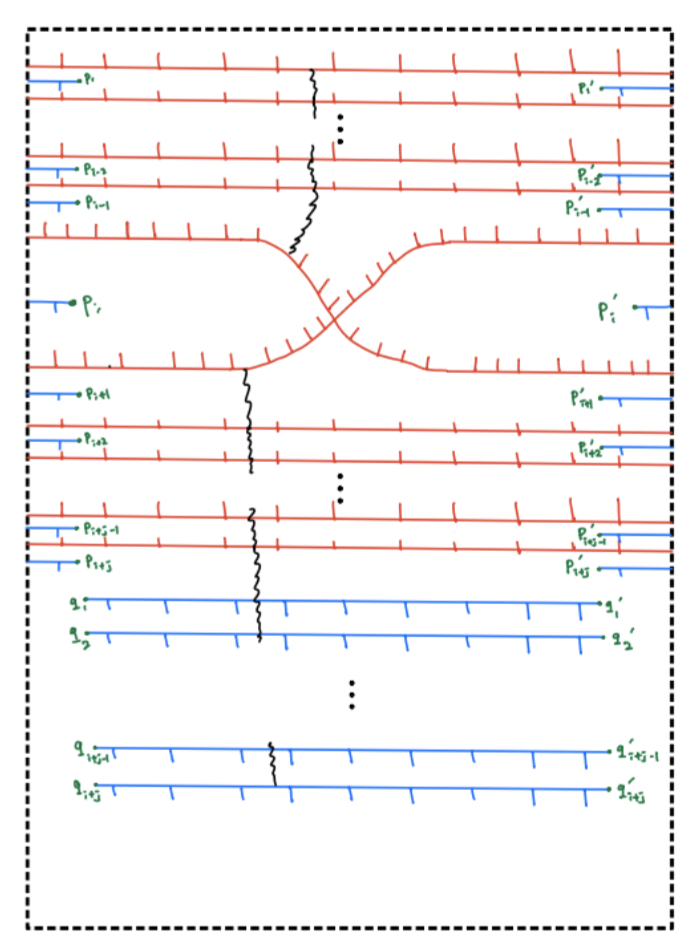
\includegraphics[width=\linewidth]{diagrams/theorem12/16.png} % Adjust the width as needed
    \caption{Your caption here}
    \label{fig:your-label}
\end{figure}